\documentclass{article}

%% PAQUETES

% Paquetes generales
\usepackage[margin=2cm, paperwidth=210mm, paperheight=297mm]{geometry}
\usepackage[spanish]{babel}
\usepackage[utf8]{inputenc}
\usepackage{gensymb}

% Paquetes para estilos
\usepackage{textcomp}
\usepackage{setspace}
\usepackage{colortbl}
\usepackage{color}
\usepackage{color}
\usepackage{upquote}
\usepackage{xcolor}
\usepackage{listings}
\usepackage{caption}
\usepackage[T1]{fontenc}
\usepackage[scaled]{beramono}

% Paquetes extras
\usepackage{amssymb}
\usepackage{float}
\usepackage{graphicx}
\usepackage{url}
\usepackage{enumerate}
\usepackage{color}

%% Fin PAQUETES


% Definición de preferencias para la impresión de código fuente.
%% Colores
\definecolor{gray99}{gray}{.99}
\definecolor{gray95}{gray}{.95}
\definecolor{gray75}{gray}{.75}
\definecolor{gray50}{gray}{.50}
\definecolor{keywords_blue}{rgb}{0.13,0.13,1}
\definecolor{comments_green}{rgb}{0,0.5,0}
\definecolor{strings_red}{rgb}{0.9,0,0}

%% Caja de código
\DeclareCaptionFont{white}{\color{white}}
\DeclareCaptionFont{style_labelfont}{\color{black}\textbf}
\DeclareCaptionFont{style_textfont}{\it\color{black}}
\DeclareCaptionFormat{listing}{\colorbox{gray95}{\parbox{16.78cm}{#1#2#3}}}
\captionsetup[lstlisting]{format=listing,labelfont=style_labelfont,textfont=style_textfont}

\lstset{
	aboveskip = {1.5\baselineskip},
	backgroundcolor = \color{gray99},
	basicstyle = \ttfamily\footnotesize,
	breakatwhitespace = true,   
	breaklines = true,
	captionpos = t,
	columns = fixed,
	commentstyle = \color{comments_green},
	escapeinside = {\%*}{*)}, 
	extendedchars = true,
	frame = lines,
	keywordstyle = \color{keywords_blue}\bfseries,
	language = Oz,                       
	numbers = left,
	numbersep = 5pt,
	numberstyle = \tiny\ttfamily\color{gray50},
	prebreak = \raisebox{0ex}[0ex][0ex]{\ensuremath{\hookleftarrow}},
	rulecolor = \color{gray75},
	showspaces = false,
	showstringspaces = false, 
	showtabs = false,
	stepnumber = 1,
	stringstyle = \color{strings_red},                                    
	tabsize = 2,
	title = \null, % Default value: title=\lstname
	upquote = true,                  
}

%% FIGURAS
\captionsetup[figure]{labelfont=bf,textfont=it}
%% TABLAS
\captionsetup[table]{labelfont=bf,textfont=it}

% COMANDOS

%% Titulo de las cajas de código
\renewcommand{\lstlistingname}{Código}
%% Titulo de las figuras
\renewcommand{\figurename}{Figura}
%% Titulo de las tablas
\renewcommand{\tablename}{Tabla}
%% Referencia a los códigos
\newcommand{\refcode}[1]{\textit{Código \ref{#1}}}
%% Referencia a las imagenes
\newcommand{\refimage}[1]{\textit{Imagen \ref{#1}}}


\begin{document}
\pagenumbering{roman}
\setcounter{page}{5}



% TÍTULO, AUTORES Y FECHA
\begin{titlepage}
	\vspace*{\fill}
	\begin{center}
		\Large 75.42 Taller de Programación I \\
		\Huge TP N°5: Archivos Ubicuos \\
		\bigskip\huge\textit{Grupo 04} \\
		\bigskip\bigskip\bigskip\bigskip\bigskip\bigskip
		\bigskip\bigskip\bigskip\bigskip\bigskip\bigskip\bigskip
		\medskip\huge\textit{``Documentación Técnica''} \\
		\date{}
	\end{center}
	\vspace*{\fill}
\end{titlepage}
\newpage




% ÍNDICE
\tableofcontents
\newpage
\pagenumbering{arabic}




% REQUERIMIENTOS DE SOFTWARE
\section{Requerimientos de software}
	
	Se listan a continuación los distintos requerimientos mínimos y necesarios para poder compilar, desarrollar, probar y depurar las aplicaciones que conforman al proyecto:
	\medskip

	\begin{itemize}
	\itemsep=5pt \topsep=0pt \partopsep=0pt \parskip=0pt \parsep=0pt

		\item \textit{Sistemas operativos}: GNU/Linux (x86 y x86-64, distribuciones Linux basadas en RPM y DEB);

		\item \textit{Controlador de versiones}\footnote{Este requerimiento es de caracter opcional ya que solo es necesario en caso de desear clonar el proyecto desde el repositorio del grupo.}: GIT (\url{http://git-scm.com/});

		\item \textit{Compilador}: g++ (\url{http://gcc.gnu.org/});

		\item \textit{Herramientas}: Make (\url{http://www.gnu.org/software/make/}).

	\end{itemize}
\bigskip




% DESCRIPCIÓN GENERAL
\section{Descripción general}

	[ Colocar texto aquí ]
\bigskip




% APLICACIÓN SERVIDOR
\section{Aplicación \textit{Servidor}}

	[ Colocar texto aquí (descripción general)]
\bigskip



% APLICACIÓN SERVIDOR - Clases
\subsection{Clases}

	[ Colocar texto aquí ]
\bigskip



% APLICACIÓN SERVIDOR - Diagramas UML
\subsection{Diagramas UML}


% Figura 1
\begin{figure}[h]
	\centering
	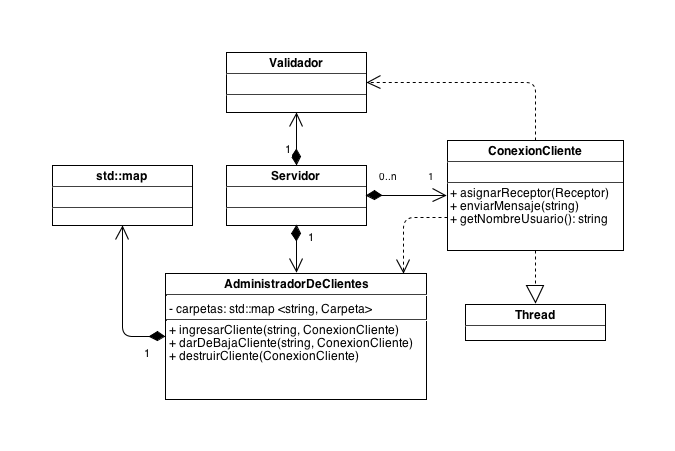
\includegraphics[width=0.85\textwidth]{images/Diagrama-modelo-servidor-parte1.png}
	\caption{Diagrama de clases principal del servidor.}
\end{figure}
\bigskip

\newpage

% Figura 2
\begin{figure}[h]
	\centering
	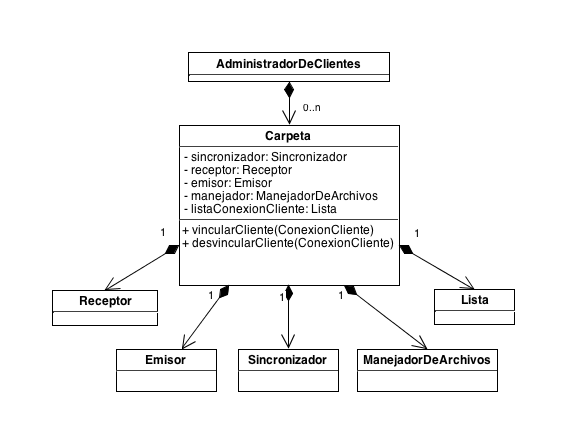
\includegraphics[width=0.72\textwidth]{images/Diagrama-modelo-servidor-parte2.png}
	\caption{Diagrama que muestra la jerarquía de clases principales.}
\end{figure}
\bigskip


% Figura 3
\begin{figure}[h]
	\centering
	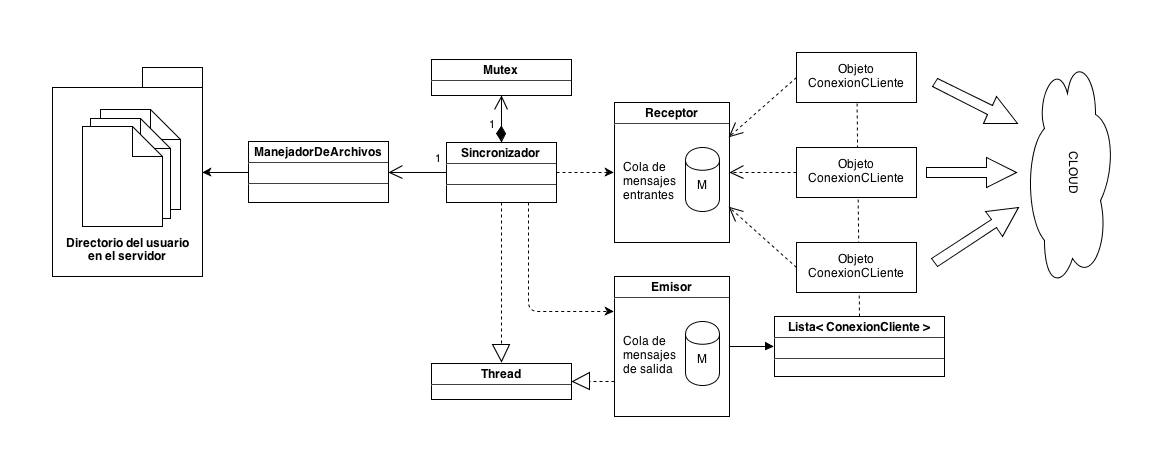
\includegraphics[width=1.0\textwidth]{images/Diagrama-modelo-servidor-parte3.png}
	\caption{Diagrama de representación de una Carpeta\\ con clientes conectados.}
\end{figure}
\bigskip






% APLICACIÓN SERVIDOR - Descripción de archivos  protocolos
\subsection{Descripción de archivos  protocolos}

	[ Colocar texto aquí ]
\bigskip




% APLICACIÓN CLIENTE
\section{Aplicación \textit{Cliente}}

	[ Colocar texto aquí (descripción general)]
\bigskip



% APLICACIÓN CLIENTE - Clases
\subsection{Clases}

	[ Colocar texto aquí ]
\bigskip



% APLICACIÓN CLIENTE - Diagramas UML
\subsection{Diagramas UML}


% Figura 4
\begin{figure}[h]
	\centering
	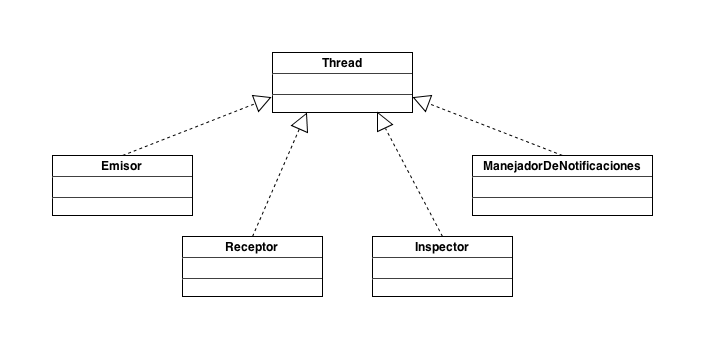
\includegraphics[width=0.85\textwidth]{images/Diagrama-modelo-cliente-threads.png}
	\caption{Diagrama de clases que indica aquellas que son un Thread.}
\end{figure}
\bigskip


% Figura 5
\begin{figure}[h]
	\centering
	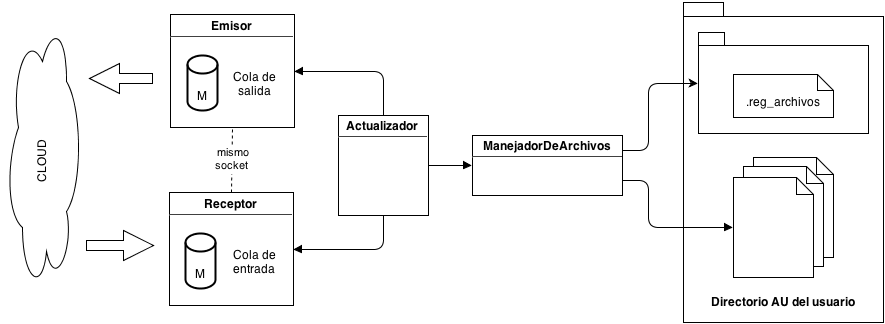
\includegraphics[width=1.0\textwidth]{images/Diagrama-modelo-cliente-actualizacion.png}
	\medskip
	\caption{Diagrama de clases que muestra de que forma se \\ relacionan en el proceso de actualización inicial.}
\end{figure}
\bigskip


% Figura 6
\begin{figure}[h]
	\centering
	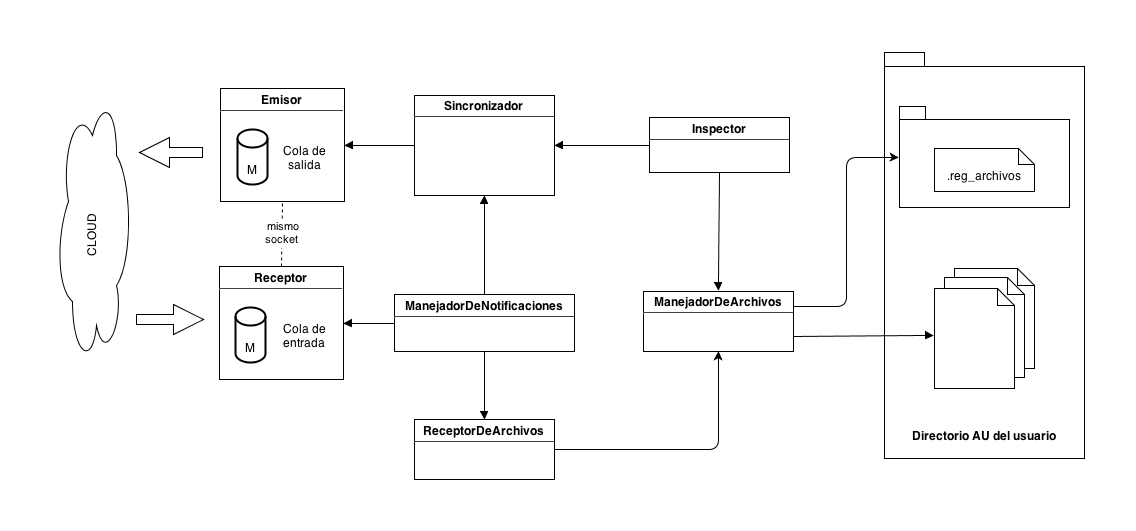
\includegraphics[width=1.0\textwidth]{images/Diagrama-modelo-cliente.png}
	\caption{Diagrama de clases que muestra de que forma se \\ relacionan en el proceso de sincronizacion.}
\end{figure}
\bigskip



% APLICACIÓN CLIENTE - Descripción de archivos  protocolos
\subsection{Descripción de archivos  protocolos}

	[ Colocar texto aquí ]
\bigskip




% PROGRAMAS INTERMEDIOS Y DE PRUEBA
\section{Programas intermedios y de prueba}

	[ Colocar texto aquí ]
\bigskip




% CODIGO FUENTE
\section{Código Fuente}

	[ Colocar texto aquí ]
\bigskip


\end{document}
